\section{Introduction}
Efficiently identifying relations between companies based on 10k filings is an interesting and important task.
The automatic extraction of such relationships from massive data collections allows analysts to use this kind of information in their business analysis.
The FEIII Challenge 2017\footnote{\url{https://ir.nist.gov/feiii/}} addresses this problem which is located exactly at the intersection of finance and big data.
Using 10-K and 10-Q filings the challenge consists of identifying all sentences that contain the relationships between the filing financial entity and another financial entity.
In a subsequent step the resulting triples consisting of financial entity mentions, role keywords, and their contextual text should be ranked in a way, that triples which contain relevant knowledge in financial sense are ranked to top positions.
During our approach, we focus exclusively on the texts (triples) and refrain from enriching the data set with additional information such as revenue streams and other information.
In this way, we want to make sure that we focus on the core problem and not add further sources of error through the integration of additional data.
We found that one of the main difficulties is that the relatively small dataset of 1000 documents is not sufficiently large for many of the machine learning approaches we tried. 
Aggravating is that the already small amount of data is very unbalanced regarding the contained roles and the tendency to relevant and highly relevant ratings.
Thus, X, Y, Z expert ratings exist for the roles A, B, C, while for the roles G, H, J there are only X, X, and X ratings.  
In addition, there is a tendency for experts to frequently categorize documents as relevant.
Another problem stems from the fuzzy definition of ``relevance'' term.
Here it was often not clear what exactly the relevance concept refers to.

Despite these difficulties we were able to achieve an overall normalized discounted cumulative gain (NDCG) score of 98\%
% from webpage: Given a 10-K filing, an analyst asks, does Company Y, mentioned in this filing, play the role R with respect to filing Company X? Rather than simply answering "yes" or "no", a system responds by providing all the mentions of Company Y in Company X's 10-K filing, with context sentences. These triples are then in ordered by the likelihood that the context accurately defines the relationship or role R between X and Y.

\section{Description of the Data}
The dataset provided for this challenge is comprised of almost 1000 triples extracted from 25 10-K and 10-Q filings, which describe a relationship (role) between the filing company and a mentioned financial entity.
Relationships are limited to ten predefined roles, namely \textit{affiliate}, \textit{agent}, \textit{counterpart}, \textit{guarantor}, \textit{insurer}, \textit{issuer}, \textit{seller}, \textit{servicer}, \textit{trustee}, and \textit{underwriter}.
Additional information, such as the context a triple was extracted from and supplementary meta-data about the entities are contained as well.

Experts labelled the relevance of triples as \textit{irrelevant}, \textit{neutral}, \textit{relevant}, or \textit{highly relevant}.
Depending on the context, relevance may be understood as an indicator for potential impact a relationship might have on the business of the filing company. 


\subsection{Inter Annotator Agreement}
The quality of annotations is estimated using Cohen's kappa. The inter annotator agreement (IAA) between two experts is defined as
$$
\kappa = \frac{p_0-p_e}{1-p_e},
$$
where $p_0$ is the proportion of labels with agreement, and $p_e$ the statistical chance of random agreement.

\begin{figure}
	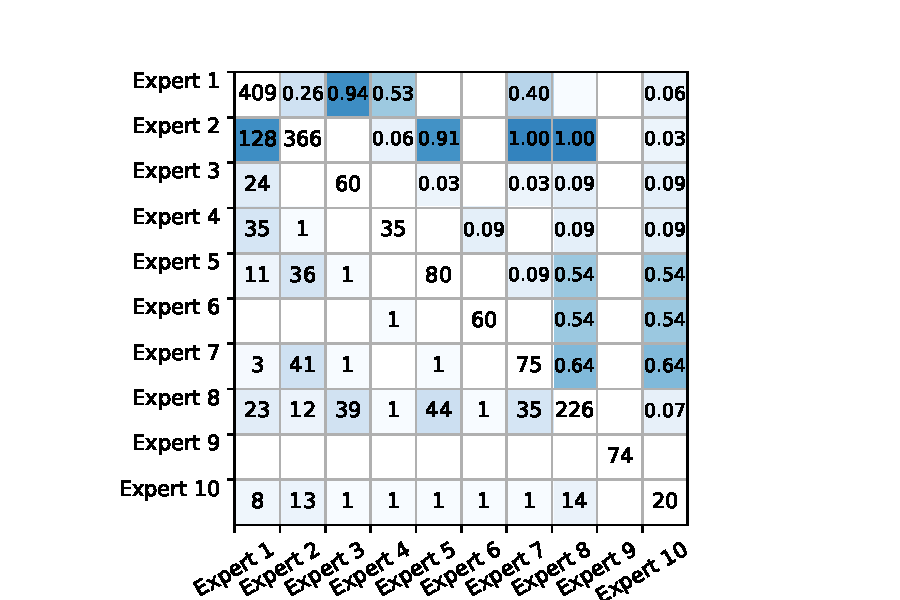
\includegraphics[width=0.7\linewidth]{iaa}
	\caption{$\kappa$ IAA (upper triangular matrix), number of commonly rated triples (lower triangular matrix), and number of ratings (diagonal matrix)}
	\label{fig:iaa}
\end{figure}

\Fref{fig:iaa} shows the $\kappa$ for each pair of experts, as well as the number of overlapping labels. Most triplets (60\%) aren't represented in this figure, since they only received a rating by one expert and very few by more than two. The weighted average of $\overline{k}<0.5$ and few overlapping annotations are not ideal for a reliable development and evaluation of a system.

\subsection{Preparing the Dataset}
Our ranking model takes the three sentences triples are extracted from as input to predict its relevance.
Especially due to the limited size of the dataset, normalising the text is an important first step, thus the strings are lower-cased and tokenised. 
Furthermore, tokens are lemmatised using the language model provided by SpaCy\footnote{\url{https://spacy.io/}}.
Based on the normalised tokens of the entire training set, a dictionary is constructed.

We used EDGAR\footnote{\url{https://www.sec.gov/edgar/aboutedgar.htm}} to retrieve the full original filings. In total, these documents contain over 60k sentences (2M words), on which we train an embedding.

As mentioned above, experts may not always agree in their rating, therefore each triple's rounded average rating is considered for all experiments.
The four rating categories are mapped to numerical values (1-4).

\section{Ranking Model}
Developing a ranking model that estimates the relevance based on text assumes the presence of phrases mostly distinct for each category.
We consider three concepts to numerically represent the three sentences as input to our model, namely \textit{bag-of-words} (BOW), an \textit{embedding} (EMB), and \textit{syntax features} (SYN).

The bag-of-words representation is constructed as follows. 
Before building the dictionary, n-grams of length one to three are formed from lemmatised tokens. 
A filter removes most and least frequent terms to reduce the feature space. To emphasise n-grams most meaningful for class distinction, the inverse document frequency (IDF) is calculated by virtually putting all texts with the same rating in one ``document''. 
Each sentence then is encoded as a bag-of-words vector where the respective positions contain the IDF weighted by the corresponding term frequency in the sentence.

Difficulties with previously unseen examples might arise from the limited size of the dictionary for the BOW.
Therefore, we created a doc2vec\cite{le2014distributed} embedding from 25 of the original full text filings on a sentence basis using the implementation by Gensim\cite{gensim}.
The vectors induced for each of the three sentences for a sample are concatenated and padded or truncated if necessary.
The resulting vector is used as input to the model.

Lastly, to provide a language independent approach, we created a selection of syntax-based features.
Following the gini impurity metric and information gain, features like the ratio of upper-case words and numbers or the number of dollar signs and word repetitions appear to be most meaningful for classification.

For each role, an ensemble of logistic regression models is trained to classify the sentences into four relevance categories.
For some roles, the number of samples is to small to train a reasonable model.
It was found, that training on the entire set, disregarding the roles, results in similar or even better performance.
Whereas a logit model is a good choice for the BOW and embeddings, since it may not as quickly affected by over-fitting, it performs badly on syntax features.
Random forests have shown promising results in this case, but are not applied to BOW as it might be more prone to favouring a small number of n-grams and thus not generalise well.

The predictions of the model for previously unseen samples return a softmax score for each of the four categories.
One could simply take the argmax as a categorical rating, but since the goal is to create a ranking, using the weighted sum of the confidence scores leads to better results.

\section{Evaluation and Conclusion}
The system's performance is measured by the Normalised Discounted Cumulative Gain (NDCG). The rank at position $p$ is calculated by
\begin{equation}
NDCG_p = \frac{DCG_p}{IDCG_p},\;
DCG_p = rel_1 + \sum_{i=2}^{p} \frac{rel_i}{\log_2(i+1)}
\end{equation}
where $DCG_p$ is the Discounted Cumulative Gain (DCG) when ordering items based on a given score, $IDCG_p$ the ideal DCG, and $rel_i$ the relevance of an item at position $i$ as depicted by the experts.

For the cross-evaluation, the labelled samples are split into a training and test set.
Triples in both sets do not share the filings they were extracted from and the distribution of ratings is roughly stratified.
As mentioned before, for each experiment, eleven models are trained. One over samples ignoring the role and one for each subset restricted to a role.
Predictions are only performed on each role's test sets.
Scores for the ranking are either continuous or categorical as described above.

\begin{table}
	\caption{Experimental results for bag-of-words (BOW), embedding (EMB), syntax (SYN) features, and ensemble}
	\label{tab:results}
	\begin{tabular}{lcccc}
		\toprule
		Approach & NDCG & $\sigma ($NDCG$)$ & F1-Score &  $\sigma ($F1$)$\\
		\midrule
		Baseline (random) & 0.87 & 0.07 & - & - \\
		Baseline (worst)  & 0.73 & 0.13 & - & - \\
		\midrule
		BOW & \textbf{0.98} & 0.03 & 0.73 & 0.27\\
		EMB & 0.92 & 0.07 & 0.41 & 0.16\\
		SYN & 0.94 & 0.06 & 0.43 & 0.26 \\
		BOW+EMB+SYN& 0.93 & 0.06 & 0.46 & 0.22\\
		\bottomrule
	\end{tabular}
\end{table}

In \fref{tab:results} lists the mean NDCG scores and the standard deviation ($\sigma$).
For comparison we take a baseline of the worst possible ranking (inverse order of the ideal ranking) and the average of multiple random rankings.
Models that disregard roles during training consistently outperform the others by a margin of over 0.05 and are not listed here.
Furthermore, the calculated continuous ranking score is able to add another slight improvement over the categorical score.

The BOW model performed best in our experiments, the EMB and SYN models show similar results. 
Training a model on text usually requires a reasonably large corpus.
With the data at hand we had to pay close attention to the selection of features, since seemingly very specific terms are likely to negatively affect the model's ability to classify unseen samples.

Looking at the performance of the classification task itself, measured by the F1-Score, the EMB model has the smallest standard deviation across multiple runs of the evaluation.
Since the embedding is trained on a significantly larger dataset, slight deviations in the input are tolerated.
In the general case, this model might perform better than the others.

Combining the features did not produce an improved model. The soft-voted ensemble of all classifiers shows similar results as EMB and SYN alone.


%\begin{figure}
%	\begin{subfigure}[t]{0.5\linewidth}
%		\centering
%		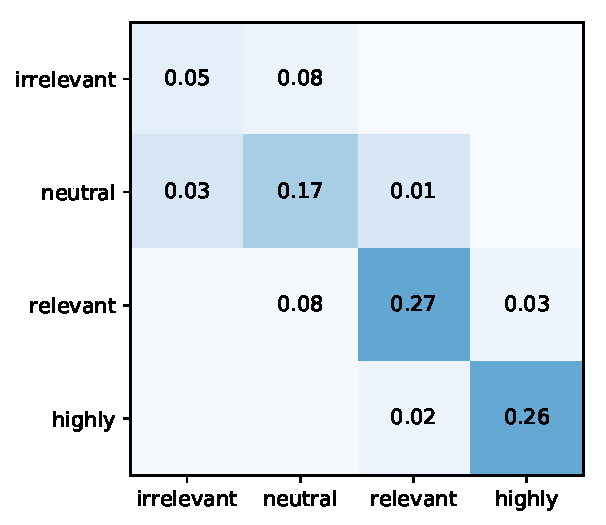
\includegraphics[width=\linewidth]{conf_full}
%		\caption{Trained on all samples}
%	\end{subfigure}%
%	~ 
%	\begin{subfigure}[t]{0.5\linewidth}
%		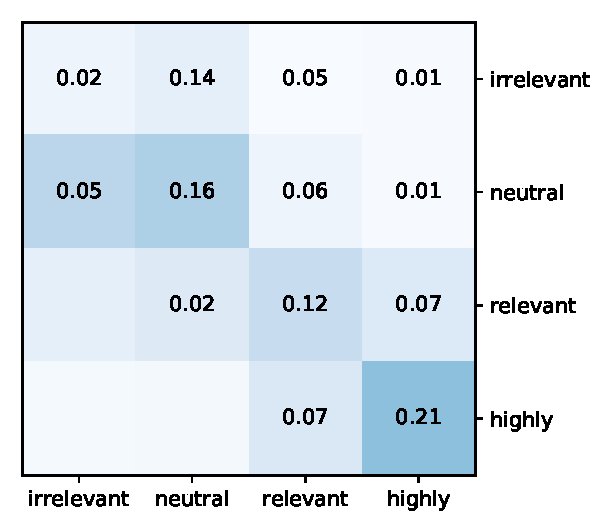
\includegraphics[width=\linewidth]{conf_role}
%		\caption{Trained on role samples}
%	\end{subfigure}
%	\caption{Normalised aggregated confusion matrices for the model with different training sets}
%	\label{fig:confmatrix}
%\end{figure}
%


%\begin{table}
%	\caption{Experimental results for bag-of-words (BOW), embedding (EMB), syntax (SYN) features}, and ensemble (ENS)
%	\label{tab:results}
%	\begin{tabular}{lcc}
%		\toprule
%		Approach & NDCG & $\sigma ($NDCG$)$\\
%		\midrule
%		Baseline (random) & 0.87 & 0.07\\
%		Baseline (worst) & 0.73 & 0.13\\
%		\midrule
%		%F1 full 0.73 std=0.27
%		%F1 role 0.49 std=0.17
%		BOW, full set, categorical & 0.97 & 0.04 \\
%		BOW, role based, categorical & 0.92 & 0.07  \\
%		BOW, full set, continuous & \textbf{0.98} & 0.03 \\
%		BOW, role based, continuous & 0.93 & 0.07 \\
%		\midrule
%		% F1 full 0.41 std=0.16
%		% F1 role 0.38 std=0.21
%		EMB, full set, categorical & 0.91 & 0.07 \\
%		EMB, role based, categorical & 0.89 & 0.07  \\
%		EMB, full set, continuous & 0.92 & 0.07 \\
%		EMB, role based, continuous & 0.90 & 0.08 \\
%		\midrule
%		% F1 full 0.43 std=0.26
%		% F1 role 0.39 std=0.26
%		SYN, full set, categorical & 0.93 & 0.07 \\
%		SYN, role based, categorical & 0.92 & 0.07  \\
%		SYN, full set, continuous & 0.94 & 0.06 \\
%		SYN, role based, continuous & 0.92 & 0.08 \\
%		\midrule
%		% F1 full 0.46 std=0.22
%		% F1 role 0.39 std=0.20
%		ENS, full set, categorical & 0.93 & 0.06 \\
%		ENS, role based, categorical & 0.91 & 0.07  \\
%		ENS, full set, continuous & 0.93 & 0.06 \\
%		ENS, role based, continuous & 0.92 & 0.07 \\
%		\bottomrule
%	\end{tabular}
%\end{table}
